\chapter{Classification Method} \label{chap:kitt_nn}
Own implementation of the chosen classification algorithm is one of the main objectives of the thesis. Principles of feedforward neural networks, based on the perceptron idea (see \cref{sec:intro_to_nn}), are used for developing the new framework.

As the first part of the study is devoted to the development of a new network pruning algorithm, besides some standard functions, the new framework implementation must meet the following requirements:

\begin{enumerate}
\item ability to remove a synapse in a network and then to retrain the network of a new structure
\item realization of a learning algorithm for a pruned network
\item visualization of the learning process in real time (an extra property)
\end{enumerate}

In this thesis, the implemented neural network framework is called \textbf{kitt\_nn}. The implementation is described in \cref{sec:implementation_of_nn}.

\section{Network Design Choices} \label{sec:network_design_choices}
It is chosen to use the \textit{feedforward} neural network idea, so none of the neurons can lead to the same or any of the previous layers and is connected to all neurons in the following layer by default (\cref{img:neural_net}).

\begin{figure}[H]
  \centering
  \includegraphics[width=0.9\textwidth]{neural_net.png}
  \caption{Feedforward neural network}
  \label{img:neural_net}
\end{figure}

As the sizes of input and output layers are determined by a chosen dataset, the network structure is utterly defined by:
\begin{itemize}
\item number of hidden layers
\item number of neurons in each of the hidden layers
\end{itemize}

A learning algorithm is assigned to an already initialized network afterwards. Standard \textit{backpropagation} is used (described in the following \cref{sec:learning_algorithm}).

The forward propagation is discussed also as a part of the learning process in \cref{ssec:forward_propagation}. The sigmoid function given as in \cref{eq:nn_transfer_function} is used as the transfer function for computing the activities of individual neurons.

\begin{align} \label{eq:nn_transfer_function}
f(z) = \frac{1}{1 + e^{-z}}
\end{align}

Its derivative used in backpropagation for computing the errors (\cref{eq:error_backprop}) is defined as in \ref{eq:nn_transfer_function_der}

\begin{align} \label{eq:nn_transfer_function_der}
f'(z) = f(z) \cdot (1-f(z))
\end{align}

The sigmoid function maps neuron activations into $ [0.0, 1.0] $ interval. This approach is used for most of the work in this study. Additionaly, the \textit{tanh(z)} function is implemented (compared to \textit{sigmoid(z)} in \cref{img:sigmoid}), in order to test one of the pruning methods based weights sensitivity (discussed later). The \textit{tanh(z)} function maps the input \textit{z} into $ [-1.0, 1.0] $ interval.

\begin{figure}[H]
  \centering
  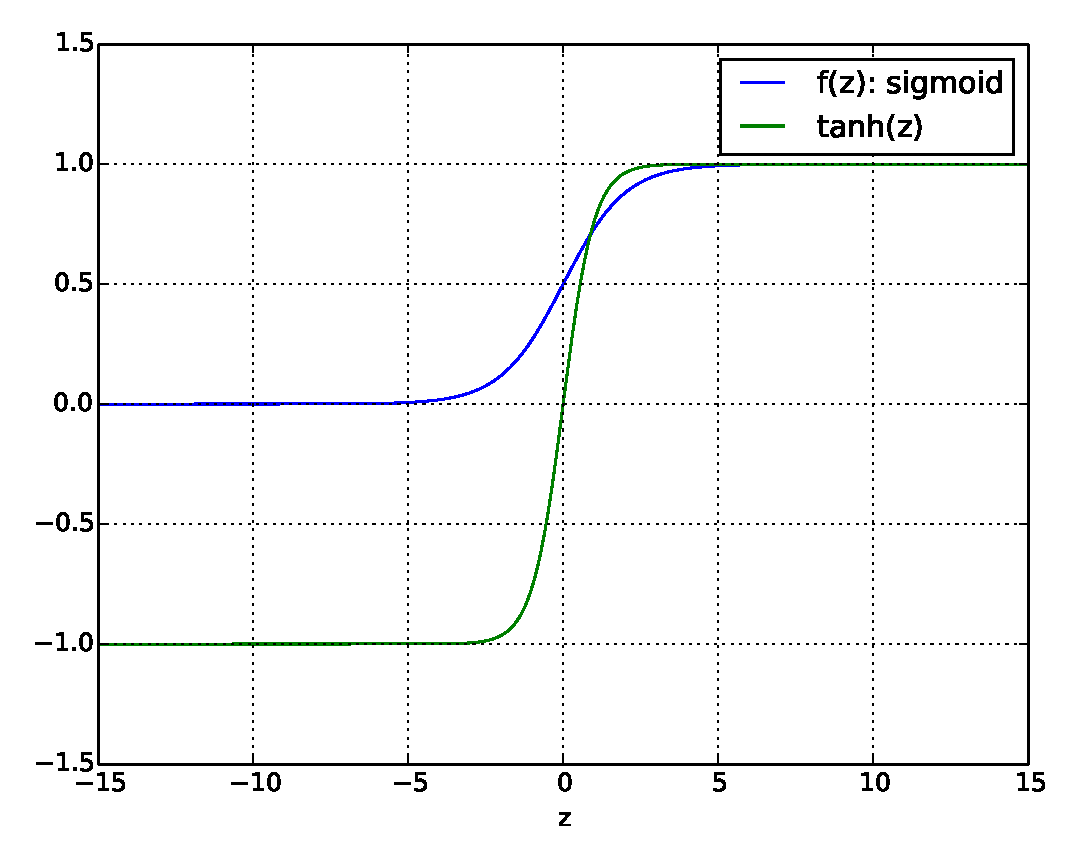
\includegraphics[width=0.7\textwidth]{transfer_functions}
  \caption{Used transfer functions: sigmoid and tanh}
  \label{img:sigmoid}
\end{figure}

\newpage
\section{Learning Algorithm} \label{sec:learning_algorithm}
In general, learning algorithms represent the part of artificial systems that makes them behave intelligently when accomplishing a specific task. In classification, the goal of learning is to fit some training data to a model, which generally means to set some parameters based on the chosen classification approach.

In case of feedforward neural networks, the learning goal is to find optimal values for two groups of parameters - \textit{weights} and \textit{biases} (described in \cref{sec:intro_to_nn}).

A popular algorithm called \textit{Backpropagation} has been chosen to deal with the learning task. The backpropagation abbreviation stands for \textit{backward propagation of errors}. The approach is based on an optimization method called \textit{Gradient Descent Algorithm (GDA)}. Method details can be found in \citep{online:nn_demystified}.

In this work, the implementation is made to be compatible with the \textit{kitt\_nn} network (\cref{sec:implementation_of_nn}) and adjusted to the needs of the developed pruning algorithm (\cref{sec:network_pruning_algorithm}). The learning process is summarized by the following flowchart \ref{img:backpropagation} and the procedure follows algorithmical steps in \citep{online:nn_demystified}.

\begin{figure}[H]
  \centering
  \includegraphics[width=1\textwidth]{backpropagation.png}
  \caption{Training process flowchart}
  \label{img:backpropagation}
\end{figure}

\begin{description}
\item[$ T_1 $] : Threshold for a terminating condition based on a learning error. If the error is reduced to be lower than this threshold, the learning process is stopped.
\item[$ T_2 $] : Threshold for a terminating condition based on number of iterations (epochs). The learning process is stopped after a specified number of epochs, no matter how successful the training has been.
\end{description}

\subsection{Using Mini-batches} \label{ssec:minibatches}
The idea of multilayer perceptrons (\cref{sec:intro_to_nn}) is described on propagating one sample through a network. However, using the matrix arithmetic, more samples can be send to the network, while activities and activations of neurons in one layer are computed at the same time for all of those samples.

This group of samples is called \textit{a mini-batch}. Using mini-batches can speed up the process, however it can bring some problems with finding the right solution by the \textit{Gradient Descent} method (evident from \cref{eq:batch_gd}). Usually, the mini-batch size is left as a training parameter. In this work, it is set to \textit{10}.

\subsection{Matrix Notation} \label{ssec:matrix_notation}
Assuming feedforward neural networks (multilayer perceptrons), the following notation is used in this study.

\begin{description}
\item[$ X $] : network input: $ m $-by-$ n $ matrix, where $ m $ is the number of samples and $ n $ is the size of one sample
\item[$ W^{(i)} $] : $ p $-by-$ r $ matrix of weights for synapses from neurons in layer $ i $ (layer of $ p $ neurons) to neurons in layer $ (i+1) $ (layer of $ r $ neurons)
\item[$ Z^{(i+1)} $] : $ r $-by-$ m $ matrix of activities for neurons in layer $ (i+1) $ (layer of $ r $ neurons), $ m $ is the number of processed samples at the same time (see \cref{ssec:minibatches})
\item[$ f() $] : transfer function (\cref{eq:nn_transfer_function})
\item[$ f'() $] : transfer function derivative (\cref{eq:nn_transfer_function_der})
\item[$ \hat{y} $] : network predicted output: $ q $-by-$ m $ matrix, where $ q $ is the number of output neurons and $ m $ is the number of processed samples ($ \hat{y} = f(Z^{(j)}) $, where $ j $ is the number of layers)
\item[$ y $] : network actual output (known targets): $ q $-by-$ m $ matrix, where $ q $ is the number of output neurons and $ m $ is the number of processed samples
\item[$ \delta^{(i)} $] : error vector of length $ p $ for $ p $ neurons of $ i^{th} $ layer
\end{description}

\subsection{Forward Propagation} \label{ssec:forward_propagation}
With reference to previous sections, the following equations are used to propagate a batch of samples $ X $ through a network and get a corresponding matrix of outputs $ \hat{y} $.

\begin{align}
Z^{(2)} = X \cdot W^{(1)}
\end{align}

\begin{align}
Z^{i+1} = a^i \cdot W^i
\end{align}

\begin{align}
a^{(i)} = f(Z^{(i)})
\end{align}

\begin{align}
\hat{y} = f(Z^{(j)})
\end{align}

\subsection{Error Calculation} \label{ssec:error_calculation}
To get an idea about how wrong the networks predictions are, the network needs a teacher. For this reason the learning is called \textit{supervised}, as there is a batch of training data with known targets. Comparing the predictions with the correct targets, one can calculate a prediction error. 

The prediction error of the propagated batch of samples is expressed as a cost function $ J $. The goal is to minimize $ J $.

\begin{align} \label{eq:cost_function}
J = \displaystyle{\sum_{k=1}^m} \frac{1}{2}(y_k - \hat{y}_k)^2
\end{align}

\subsection{Parameters Update} \label{ssec:parameters_update}
Knowing the prediction error, the goal of the learning algorithm is to update the network weights and biases in order to reduce the error for next prediction.  It is known, that some combination of the parameters makes $ J $ (\cref{eq:cost_function}) minimal. There is no chance to check all possible combinations for bigger networks, therefore \textit{GDA} is used here.

Partial derivatives $ \frac{dJ}{dw} $ for all weights $ w $ of chosen weights matrix $ W^{(i)} $ belonging to layer $ i $ are computed and set equal to zero ($ \frac{dJ}{dw} = 0 $). Applying this on a mini-batch, we get $ m $ derivatives $ (\frac{dJ}{dW^{(i)}})_k $ for $ m $ input samples. 

\textit{GDA} is then applied on the summation of these derivatives and so all examples are considered as one (\cref{eq:batch_gd}). In human language, one can understand it as every sample has a vote on how to find the minimal error and the result is obtained as a compromise.

\begin{align} \label{eq:batch_gd}
\frac{dJ}{dW^{(i)}} =  \displaystyle{\sum_{k=1}^m} (\frac{dJ}{dw})_k
\end{align}

There are three main issues (\cref{img:gda_problems}) preventing this approach from being perfect. However, as the brute force algorithm is uncomputable, this method is chosen.

\begin{figure}[H]
  \centering
  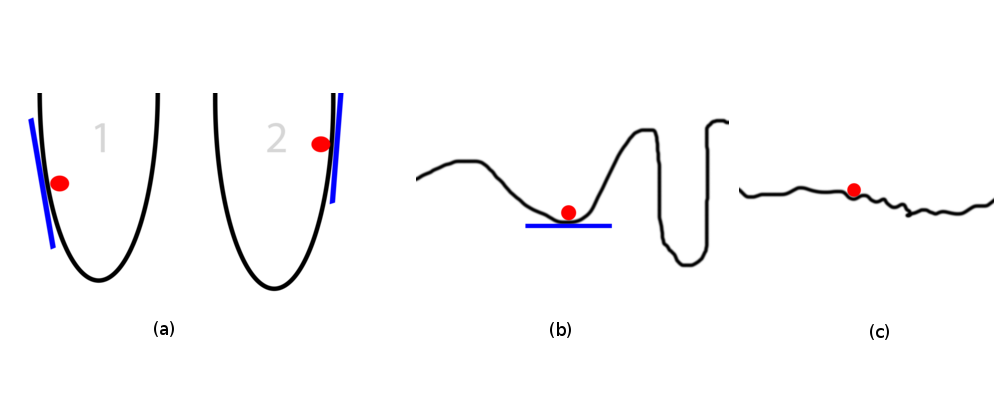
\includegraphics[width=0.85\textwidth]{gda_problems.png}
  \caption{GDA issues \citep{online:nn_demystified} (a) slopes are too big, (b) local minimums, (c) slopes are too small}
  \label{img:gda_problems}
\end{figure}


Having several layers of a network results in several weights (and biases) mattrices, while the goal is to find optimal parameters of overall network. In order to compute optimal parameters in all of the mattrices, the sum rule in differentation (\cref{eq:sum_rule}) followed by the chain rule (\cref{eq:chain_rule}) are applied.

\begin{align} \label{eq:sum_rule}
\frac{\delta}{\delta x} (u+v) = \frac{\delta u}{\delta x} + \frac{\delta v}{\delta x}
\end{align}

\begin{align} \label{eq:chain_rule}
(f \circ g)' = (f' \circ g) \cdot g'
\end{align}

Due to these properties, the error obtained at the network output (\cref{ssec:error_calculation}) is propagated backwards layer by layer through the network (\cref{eq:error_backprop}) and derivatives $ \frac{dJ}{dW^{(i)}} $ for all $ i $ layers are found (\cref{eq:part_derivative}).

\begin{align} \label{eq:error_backprop}
\delta^{(i)} = \delta^{(i+1)} \cdot (W^{(i)})^T \cdot f'(Z^{(i)})
\end{align}

\begin{align} \label{eq:part_derivative}
\frac{dJ}{dW^{(i)}} = (a^{(2)})^T \cdot \delta^{(i+1)}
\end{align}

Due to issues shown on \cref{img:gda_problems}, there are no guarranties of getting a good solution, getting a solution in a finite number of iterations and even not of getting a solution at all. However, this approach is considered as the state of the art nowadays.

In this work, it is implemented in \textit{Python}, using mostly the \textit{numpy} library for the expensive matrix operations. The implementation complies with the needs of the pruning algorithm from \cref{sec:network_pruning_algorithm} and is fully compatible with the \textit{kitt\_nn} framework for any type of data.

\section{Graphical User Interface} \label{sec:gui}
The graphical interface has been implemented as an extension for \textit{kitt\_nn} framework. It is actually not strictly needed for this study, but it provides some interesting functions worth of being introduced. Anyway, any type of visualization usually helps to understand a problem better.

\begin{figure}[H]
  \centering
  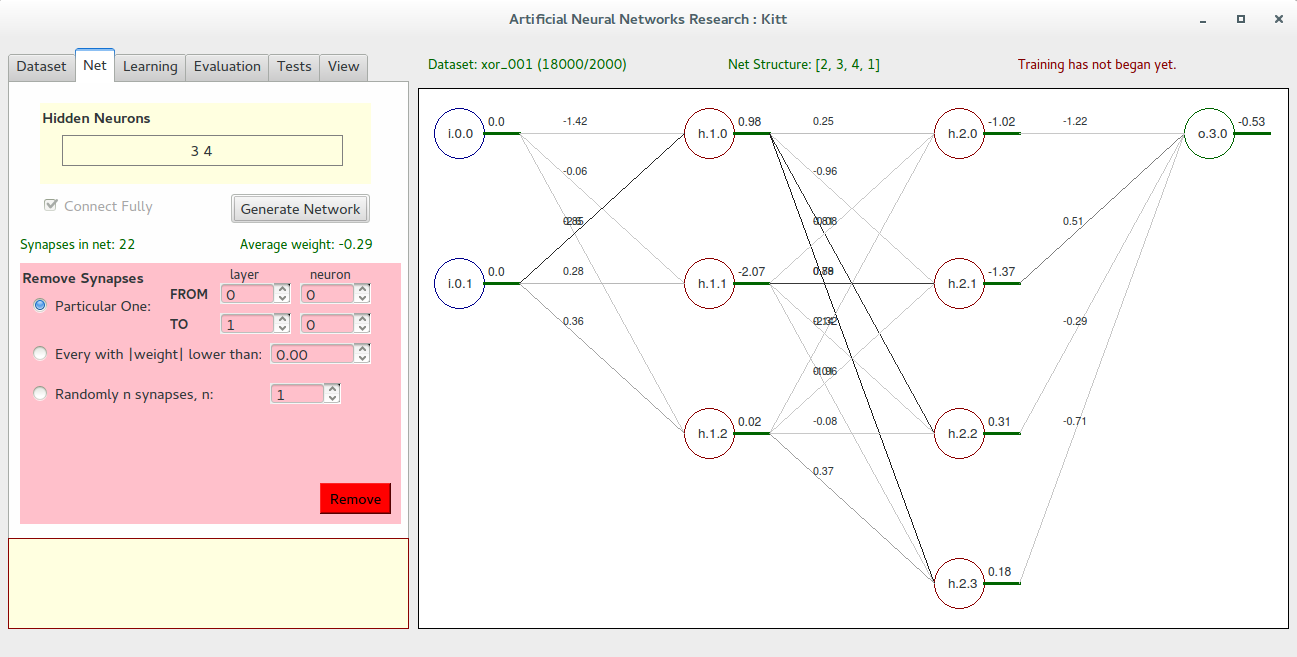
\includegraphics[width=1.0\textwidth]{gui_screen.png}
  \caption{Screenshot of the graphical user interface}
  \label{img:gui_screen}
\end{figure}

This GUI is capable of:
\begin{enumerate}
\item Loading a dataset in a specific form and, if possible, visualizing it (see XOR data in \cref{img:data_xor} for an example, this image is generated by the GUI).
\item Generating a network of any hidden structure. The input and output layers are defined by the chosen dataset. The network is then visualized (as shown in \cref{img:gui_screen}).
\item Removing synapses of the network, while the visualization is interactive with the structure changes.
\item Training the network, while the visualization is interactive, so the weights changes can be seen online.
\item Performing some tests and plotting basic evaluations.
\item Adjusting the visualization view in sense of zooming, resizing or changing colors.
\end{enumerate}

The visualization is not that useful for huge network structures, however, it can be essential at some points of the workflow. Nevertheless, it is considered as the very fist version for now and aimed to be upgraded in the future.

\newpage
\section{Network Pruning Algorithm} \label{sec:network_pruning_algorithm}
The network pruning algorithm (PA) is the novelty of this study. The state-of-the-art methods based on feedforward neural networks (see \cref{sec:intro_to_nn}) use a fully-connected structure by default. This means that each unit is connected to all units in the next layer. Hence a net structure is utterly defined just by the number of hidden layers and the number of neurons in each of those. The question is if all of the defaultly generated connections acutally take part in classification.

\subsection{Pruning Idea} \label{ssec:pa_idea}
The hypothesis is that some synapses of a fully connected feedforward network can be removed while the net's classification performance is not influenced significantly.  The problem is formulated by \cref{img:pruning_problem_formulation}.

\begin{figure}[H]
  \centering
  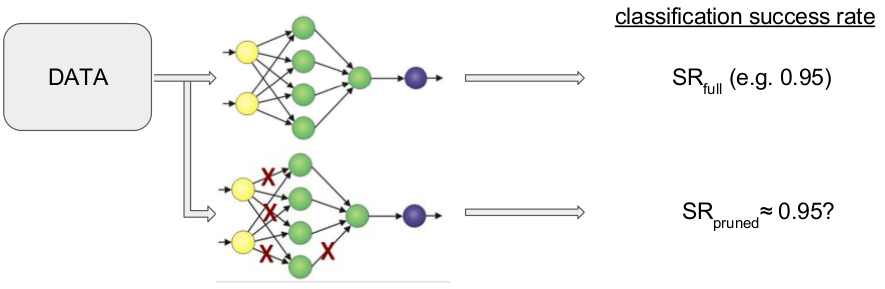
\includegraphics[width=1.0\textwidth]{pruning_problem_formulation.png}
  \caption{Pruning Algorithm: hypothesis formulation}
  \label{img:pruning_problem_formulation}
\end{figure}

The ultimate task is to distinguish the redundant synapses from the important ones. The chosen approach is to initialize a fully-connected network and train it on some data to reach as high accuracy as possible. Then some of the synapses are removed and a classification ability of the pruned net is tested. If it has not dropped, the removed synapses were redundant. The way of removing the synpases is called \textit{pruning algorithm (PA)}.

The idea behind the PA implemented in this study is based on weight changes during the network training. It is expected that a synapse, whose weight does not evolve while the network is trained, does not participate in classification at all. 

\subsection{Algorithm Realization} \label{ssec:pa_realization}
The pruning algorithm itself is an iterative process, however, as shown in \cref{img:pa_flowchart}, two important steps are done in advance.

\begin{figure}[H]
  \centering
  \includegraphics[width=0.7\textwidth]{pa_flowchart.png}
  \caption{Overall flowchart of the pruning process}
  \label{img:pa_flowchart}
\end{figure}

At first, the following variables are initialized:

\begin{description}
\item[net] : a fully-connected \textit{kitt\_nn} \textit{Network()} with an oversized structure (many hidden neurons) and randomly set weights and biases
\item[percentile] : algorithm variable, set to $ 75 $ by default
\item[percentile levels] : array of final variables, set to $ [75, 50, 20, 5, 1] $ by default
\item[required accuracy] : required classification accuracy for a chosen problem (e.g. 0.95)
\item[stability threshold] : if the classification does not improve over several learning iterations, this is the number of stable iterations to terminate the training after
\end{description}

Additionally, some standard learning parameters like the \textit{learning rate}, \textit{number of epochs} and \textit{mini-batch size} can be set and, of course, a dataset is chosen.

Once the initialization is done, the network is trained with some optimal learning parameters until it reaches the required classification success rate. As mentioned above, the algorithm is based on weight changes. Therefore, the initial weights for synapses are kept. Then, the trained network is passed to the pruning loop, which is introduced in \cref{img:pruning_algorithm}.

\begin{figure}[H]
  \centering
  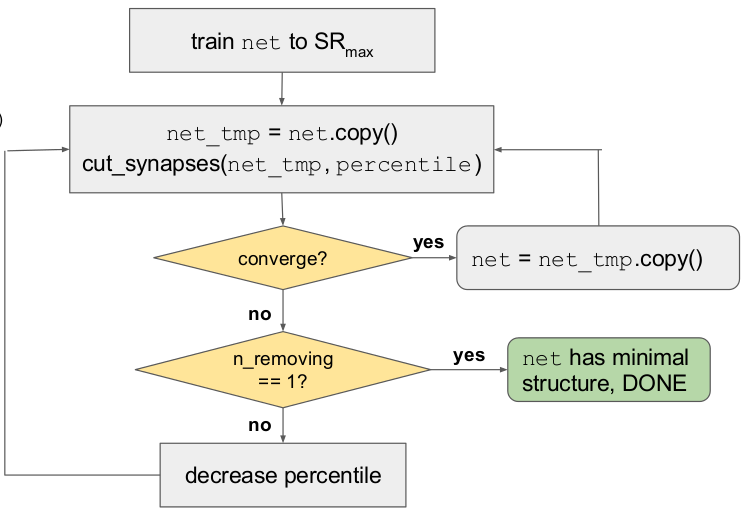
\includegraphics[width=0.9\textwidth]{pruning_algorithm.png}
  \caption{The Pruning Algorithm: initialized variables are in bold, red marked functions reffer to \ref{img:cut_synapses} and \ref{img:accuracy_kept} respectively}
  \label{img:pruning_algorithm}
\end{figure}

At first, a backup of the current network structure is made by creating a network copy. The pruning is then performed on this copy. The pruning method is shown in \cref{img:cut_synapses}.

\begin{figure}[H]
  \centering
  \includegraphics[width=0.8\textwidth]{cut_synapses.png}
  \caption{Function: removing synapses based on weight changes and current percentile value}
  \label{img:cut_synapses}
\end{figure}

As discussed above, an initial weight value had been saved for each synapse before the training. Hence, for $ n $ being the total number of synapses, weight changes $ \Delta w_i $ are known (\ref{eq:weight_change}).

\begin{align} \label{eq:weight_change}
\Delta w_i = |w\_init_i - w\_current_i|, \quad i = 1, ..., n
\end{align}

Based on these changes and on the current $ percentile $ value, a threshold ($ th $ in \cref{img:cut_synapses}) is determined. Then, all synapses with a lower change in weight than this threshold are removed, and, if there is a neuron with no connections left, it is removed as well.

If the $ percentile $ variable has been decreased such that it equals zero, the threshold is set to the minimum of all weight changes. In this case, only one synapse is then removed at a time.

After cutting some synapses, the network is checked for keeping the required classification accuracy as shown in \cref{img:accuracy_kept}.

\begin{figure}[H]
  \centering
  \includegraphics[width=0.8\textwidth]{accuracy_kept.png}
  \caption{Function: checking if the accuracy has been kept after pruning}
  \label{img:accuracy_kept}
\end{figure}

The checking is performed by evaluating the network on validation data. If the classification accuracy has dropped, the network is tried to be retrained (using training data of the dataset).

Getting back to \cref{img:pruning_algorithm}, if the classification accuracy has been kept after the pruning, the current net structure is saved and considered as a reference for the next pruning loop.

If it is not possible to retrain the pruned net and to reach the required accuracy, two possibilities arise:

\begin{enumerate}
\item Only one synapse has been removed during the last pruning step and the accuracy has been broken. This means that even this single synapse with the least change in weight is important for classification. Therefore, the pruning is stopped and the current net structure (including this last synapse) is saved as the minimal structure.
\item More synapses have been removed during the last pruning step, and this broke the accuracy. In this case, the percentile level is decreased (based on the initialized array of percentile levels) and so less synapses are removed during the next pruning iteration.

In this manner, at some point of the pruning process, the algorithm will come to removing only one synapse at once and then, sooner or later, case 1 must supervene.
\end{enumerate}

Therefore, the algorithm is finite. Moreover, it guarantees that the classification success rate does not drop. It is evaluated in detail and compared to some other approaches from \citep{article:10:pa} (also discussed in \cref{sec:pruning_algorithms}) in the results part (\cref{sec:pruning_algorithm_results}).

\subsection{Testing Datasets for the Pruning Algorithm}
Two datasets are used for testing and verification of the pruning algorithm: XOR and MNIST. Those are introduced in the following sections and the evaluation is presented in section X.

Then, the pruning algorithm is applied also on data related to this thesis: proprioceptive and tactile sensory data from a hexapod robot used for terrain classification (section X).

\subsubsection*{XOR Dataset}
This dataset relates to the well-known XOR problem defined by a thruth table (\cref{tab:xor}).

\begin{table}[H]
\centering
\caption{XOR problem definition}
\label{tab:xor}
\begin{tabular}{|c|c|c|}
\hline
$ \mathbf{x_1} $ & $ \mathbf{x_2} $ & \textbf{y} \\ \hline
0           & 0           & 0          \\ \hline
0           & 1           & 1          \\ \hline
1           & 0           & 1          \\ \hline
1           & 1           & 0          \\ \hline
\end{tabular}
\end{table}

Formulating the XOR gate as a classification problem, it is represented by two linearly inseparable classes with labels $ 0 $ and $ 1 $. In this case, each class consists of $ 1000 $ samples, which have been generated using the developed GUI (\cref{sec:gui}). The composition of the two classes in a 2D space is shown in \cref{img:data_xor}.

\begin{figure}[H]
  \centering
  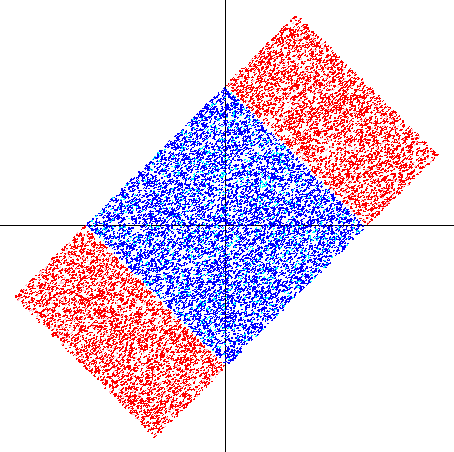
\includegraphics[width=0.4\textwidth]{data_xor.png}
  \caption{2D XOR Data illustration}
  \label{img:data_xor}
\end{figure}

The points (samples) have been generated pseudo-randomly, while it is guaranteed that the 'red' samples are distributed half-and-half between the two 'red' areas. The minimal distance between a 'blue' and a 'red' sample is $ 0.001 $ and it is possible to separate the classes using two lines.

The XOR dataset is essential for evaluation of the implemented PA, as the minimal network structure capable of solving the problem is known. There are two structures (\cref{img:xor_min}), both considered as minimal in a way. Mathematically, the version shown in \cref{img:xor_min1} creates the two lines in 2D space to separate the classes, while the second one (\cref{img:xor_min2}) creates a plane and transfers the problem into 3D.

\begin{figure}[H]
\centering
\begin{subfigure}{.5\textwidth}
  \centering
  \includegraphics[width=.5\linewidth]{xor_min1.png}
  \caption{Minimal structure 1 (2D)}
  \label{img:xor_min1}
\end{subfigure}%
\begin{subfigure}{.5\textwidth}
  \centering
  \includegraphics[width=.5\linewidth]{xor_min2.png}
  \caption{Minimal structure 2 (3D)}
  \label{img:xor_min2}
\end{subfigure}
\caption{XOR Dataset: minimal network structures}
\label{img:xor_min}
\end{figure}

The goal of the pruning algorithm is to end up with a network of one of these structures, when the network is initially oversized (evaluated in X).

\subsubsection*{MNIST Dataset}
The second testing problem is the well-known classification of handwritten digits. The dataset is provided by \citep{online:mnist}. Some examples of digit samples are shown in \cref{img:data_mnist}.

\begin{figure}[H]
  \centering
  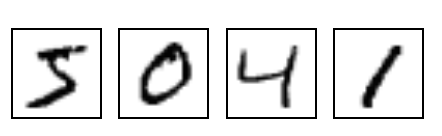
\includegraphics[width=0.7\textwidth]{data_mnist.png}
  \caption{MNIST Data illustration \citep{online:mnist}}
  \label{img:data_mnist}
\end{figure}

The dataset has a training set of $ 60,000 $ examples (later split into $ 50,000 $ training and $ 10,000 $ validation examples), and a test set of $ 10,000 $ examples. The digits have been size-normalized and centered in a fixed-size image.

In this case, the minimal network structure is not known. On the other hand, detailed results of classification accuracy for various classifiers are provided, which is good for comparison.

\subsection{Minimal Structure Utilization}
In general, only the size of the input and output layer is determined for a chosen dataset. The pruning algorithm brings an additional information about the hidden part of the network. A minimal network structure is obtained as the PA outcome. This means that all the neurons and synapses contained in the network are important for classification.

Knowing that each of these units takes a part and is not useless, one can ask what role does a single neuron/synapse have with respect to the chosen dataset.

This can be researched by tracking the connections from the input to the output layer. Based on this approach, one can find some correlations between specified parts of input vectors and a selected output class (demonstrated on a MNIST example in \cref{img:structure_util}). Evaluation on MNIST dataset is shown in section X.

\begin{figure}[H]
  \centering
  \includegraphics[width=0.7\textwidth]{min_structure_analysis.png}
  \caption{Minimal strucuture utilization explained on MNIST ('5' class sample example)}
  \label{img:structure_util}
\end{figure}